\documentclass[10pt]{article}\usepackage[margin=.65in]{geometry}\usepackage[T1]{fontenc}\usepackage{graphicx}\setlength{\parindent}{0pt}\setlength{\parskip}{7pt}\sloppy\begin{document}{\large Literal word find and same-root composition}\par Producer proof packet, 2026-11-01. Independent source-fidelity review pending.\par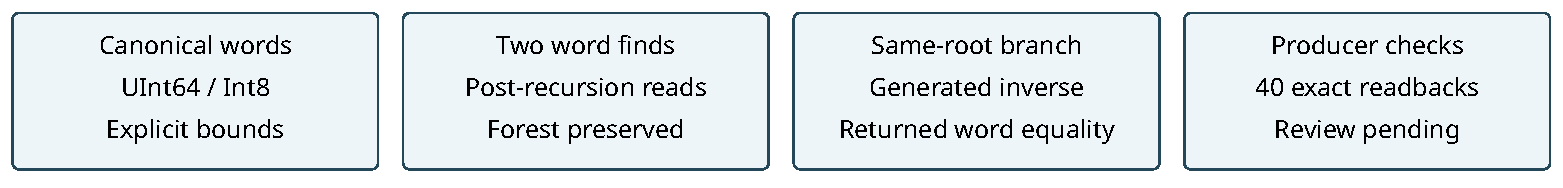
\includegraphics[width=\linewidth]{diagram.pdf}\par Result. Seven fresh Lean modules compiled. The endpoint composes two actual word-level find traces with the same-root collector branch, preserving the decoded forest and relation validity. A safe returned canonical word equals the specified canonical target word. A separate theorem supplies two word traces under the ranked-forest premises.

Checks. The native checker accepted 29 main declarations, 11 fixed producer controls and exactly 40 named axiom readbacks. The deliberately false proposition 0 = 1 failed compilation with exit 1. Three checker rejection controls passed. Local bound inputs passed the before/after hash check. No new cohort or timing data was collected; cost ratio is null.

Assumptions. Prime modulus 2 $<$ r $<$= 2\textasciicircum{}63; canonical UInt64 offsets; Int8 signs restricted to +1/-1; initial forest, valid relations and true incoming edge. The generated inverse is connected to the existing inverse theorem. The word zero test and the stored r-2 denominator are connected to field operations.

Scope. This is the modeled same-root endpoint. Distinct-root union, physical array and stack bounds, allocation, counter headroom, compiler correspondence and geometric edge production remain separate interfaces. Imported local helper caches and Mathlib dependencies were reused; only the seven named modules were freshly rebuilt. The public native API does not itself enforce all theorem premises.

Controls. Fixed modulus-7 controls cover zero constraints, inconsistent constraints, opposite/equal signs, new and existing anchors, invalid sign rejection, a nontrivial find, a second root find and the composed returned word. These are producer controls, not independent review.

Failures retained. Early drafts failed for induction-hypothesis application, namespace and simplification errors, pair syntax, product equality construction, and opaque-sign decidability. Attempt receipts are retained. The expected false theorem is separately identified by ExpectedFailure and is not counted as a failed scientific trial.

Source context. Native collector: src/cryptanalysis/three\_leads.rs at b7c231cd447823c2522b09d5390593cca46054a8, Ring through same-root edge handling. Prior reviewed derivations and literature context are in sibling next-interface-derivations and native-branch-composition packets. No novelty claim is made.

Next review. Independently map each formal branch to the pinned native source; attack canonicality, modulus and sign boundaries, post-recursion reads, generated inverses and anchor contradiction. Freshly rebuild dependencies for a stronger replay, then address the distinct-root union interface. All three assigned reviewer agents terminated with usage-limit errors; this packet remains producer-checked.
\end{document}